\chapter{Método}
\section{Estratégia \textit{bottom-up}}
A estratégia gerencial e organizacional \textit{bottom-up} foi utilizada no desenvolvimento deste projeto. 
Em função da natureza modular e orientada a comportamentos de arquiteturas reativas \cite{murphy}, a adoção deste método de gerenciamento é quase que 
uma escolha natural.
O robô foi dividido em quatro subsistemas, desenvolvidos e testados separadamente: percepção, locomoção, comunicação e navegação (que, no caso deste 
projeto, consiste no desvio de obstáculos em si). %% TODO citar a arq MOSA aqui pra falar do planejamento??
Nesta fase de implementação,  boas práticas de engenharia de software foram prioridade, buscando uma implementação que 
apresente baixo acoplamento  e alta coesão com a expectativa de desenvolver um código que possa ser facilmente entendido e reutilizado em futuros 
trabalhos afins.
Em seguida se deu a etapa de integração das partes para, a posteriori, serem feitos testes no conjunto, conforme ilustra o diagrama \ref{WBS}.

  \begin{figure}[H] %% TODO certificar se realmente é uma WBS!!!
    \centering
    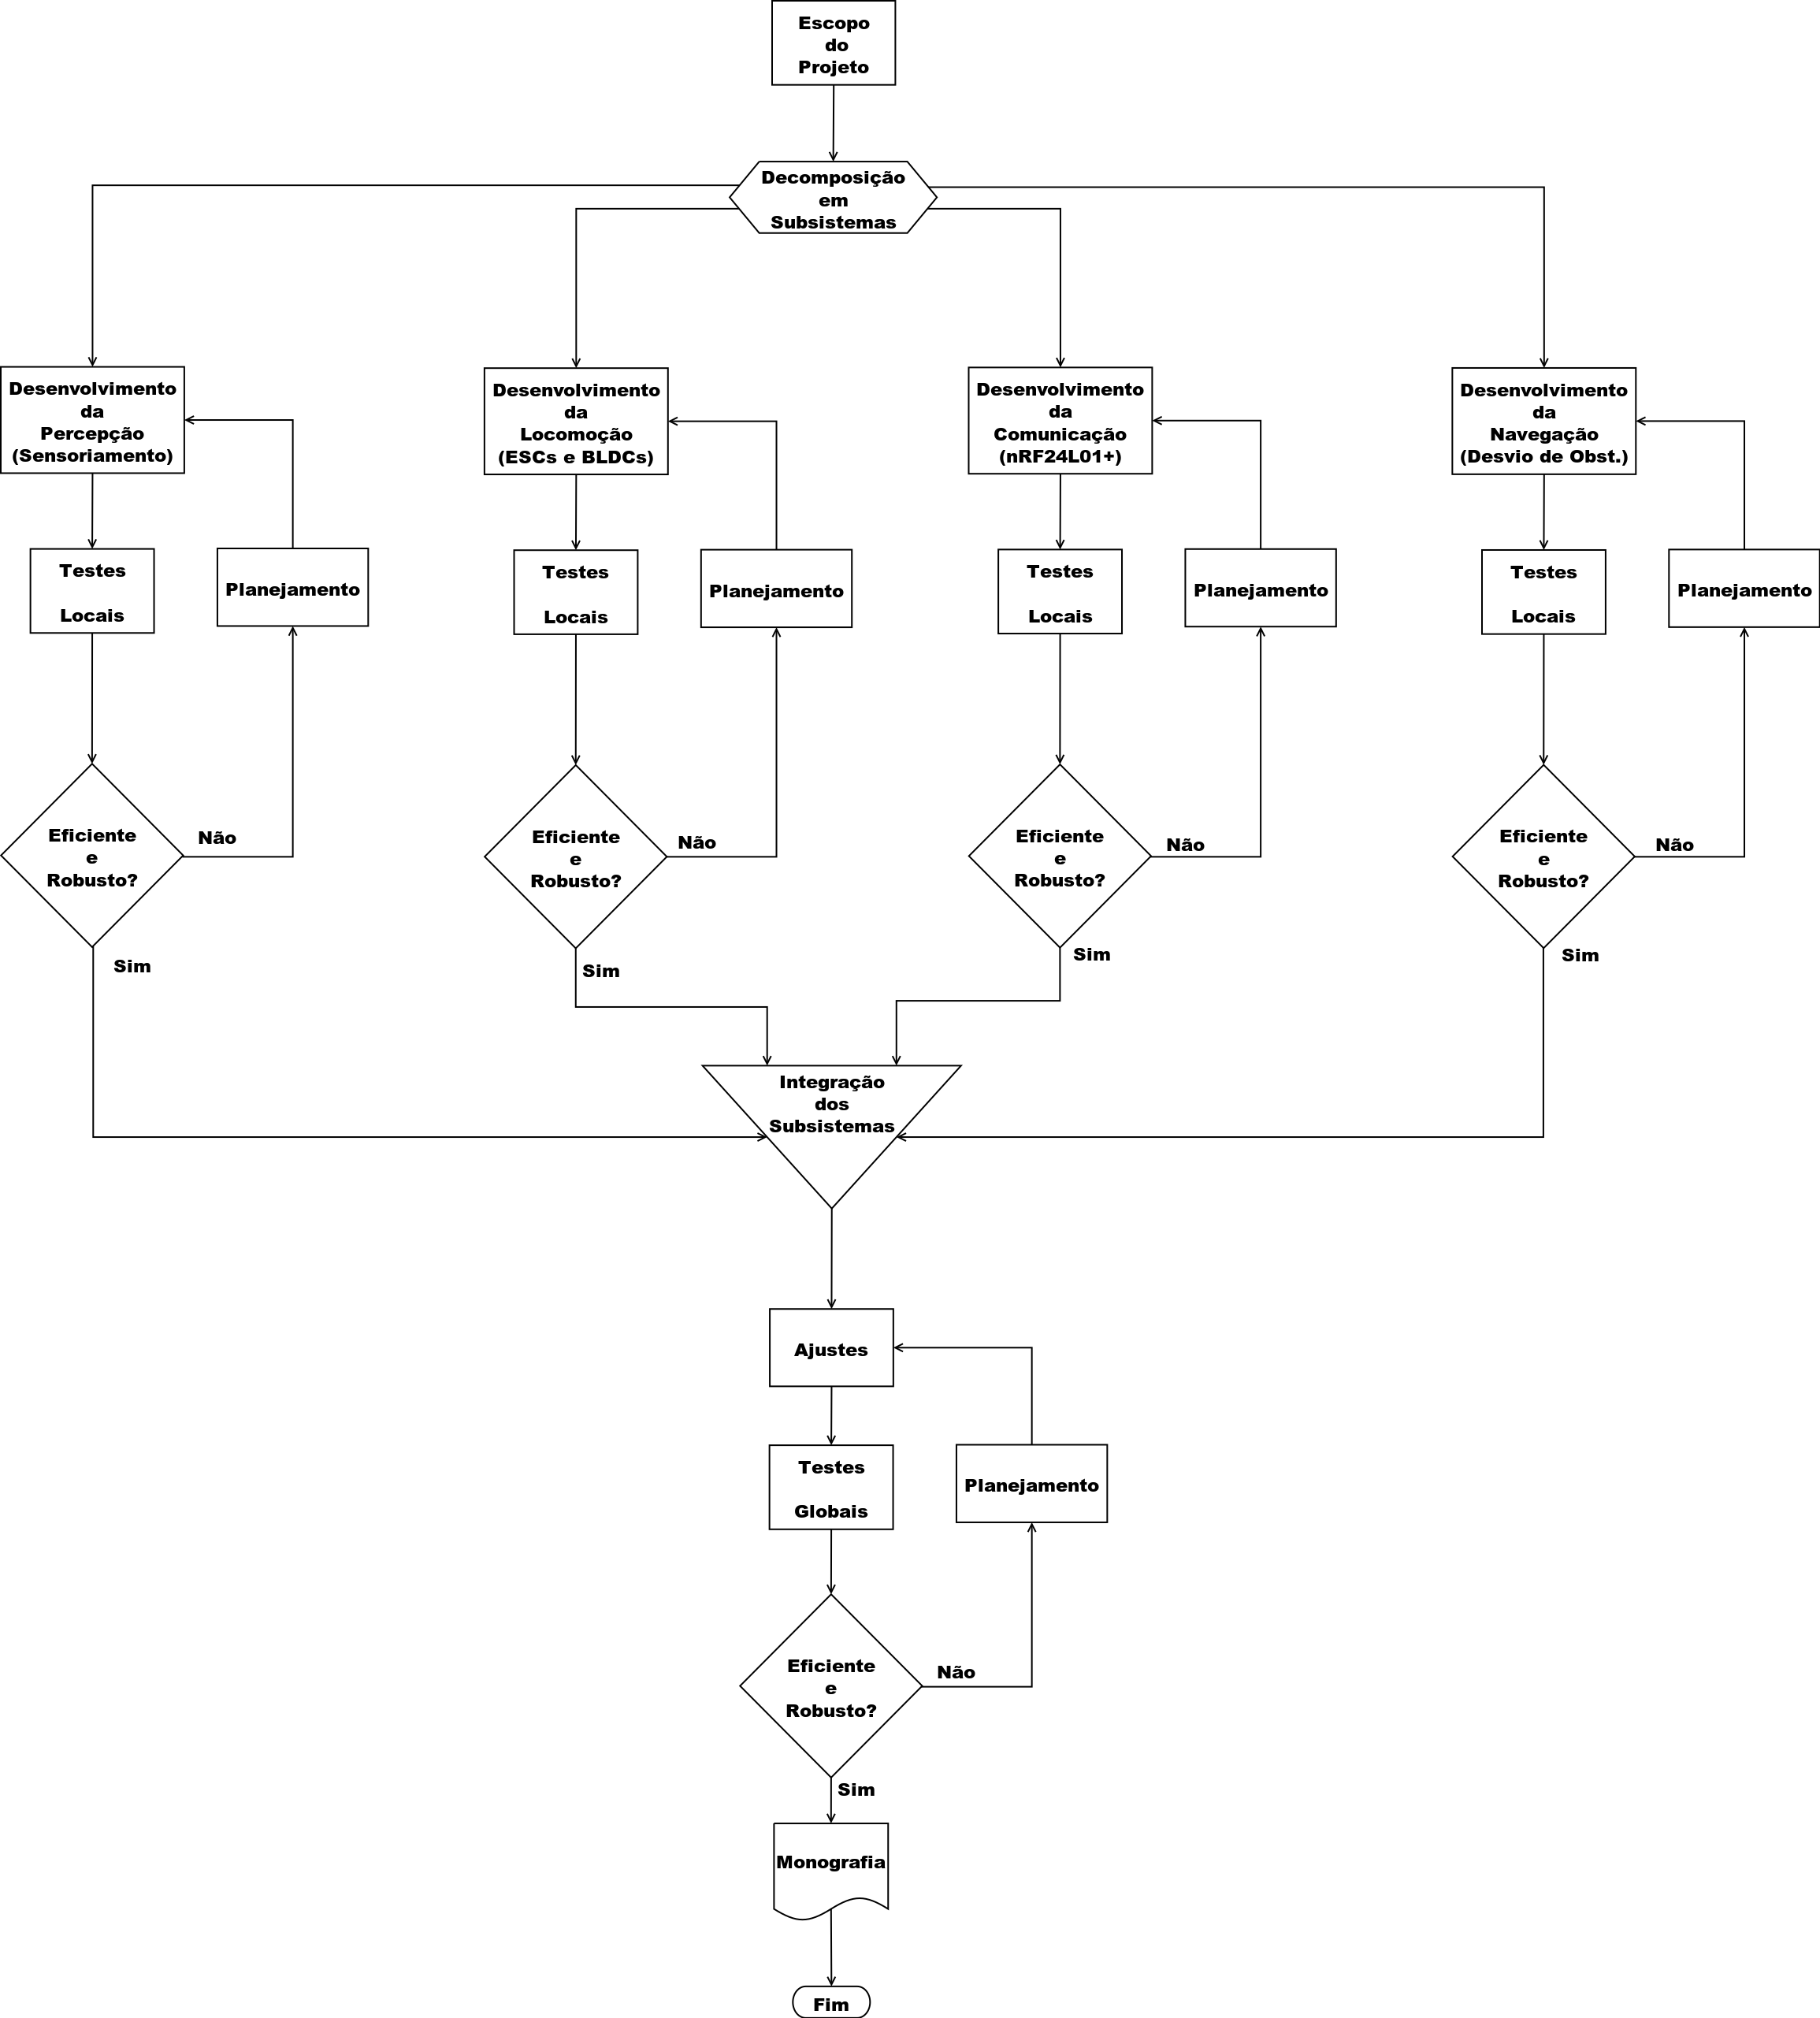
\includegraphics[width= 0.7 \linewidth]{../../Imagens/WBS.png}
    \caption{Estrutura Analítica do Projeto} %% TODO certificar se realmente é uma WBS!!!
    \label{WBS}
  \end{figure}

\section{Arquitetura Reativa} 
% creio não termos implementado uma arquitetura de subsumpção pq o robô apresenta estados internos, como transmissão via RF dos USS quando em modo de 
% navegação e o fato de poder andar caso haja mensagem informando que o SB foi acionado até 500ms antes. 

Optou-se por uma arquitetura de controle fortemente baseada nas informações sensoriais, sem delongas em processamento de sinal para ajustar os dados 
dos sensores a um modelo ou representação de mundo preconcebido. 
A razão dessa escolha é decorrência da necessidade de uma resposta rápida do sistema, vantagem da arquitetura reativa em função da sua simplicidade 
\cite{roseli}.

A latência inerente à obtenção dos dados dos sonares \cite{jones} associada à alta velocidade de operação do robô é a causa desta restrição 
temporal. % TODO não gostei da palavra temporal nesse contexto
Como é imprescindível colher dados do ambiente externo a uma taxa que dê um panorama atualizado do que está se passando ao redor do robô 
\cite{brooks}, reduzir o tempo de resposta do sistema possibilita que o desvio de obstáculos ocorra de maneira mais suave.
Haja vista que se a detecção for feita com antecedência, medidas menos bruscas podem ser adotadas; em contraste com o caso em que a latência é alta a 
ponto de que avpercepção das barreiras no caminho se dê na proximidade do veículo.

Os comportamentos implementados no robô se restringem às diferentes manobras de evasão, adotadas com base na proximidade de obstáculos dos cinco 
sensores, vide Tabela \ref{IA}. Os estímulos reguladores consistem na recepção, via RF, de um comando que incite o robô a navegar e do aval mediante 
recebimento de uma mensagem nos últimos 500ms informando se o botão de segurança foi acionado.
%TODO: as demais funções implementadas podem ser vistas como comportamentos???

\section{Subsistema de Locomoção}
Numa visão geral, temos que o Arduino é responsável por emitir um sinal de controle, modulado em largura de pulso, ao ESC.
Este, por sua vez, é incumbido de energizar os devidos enrolamentos do estator a fim de que o motor BLDC atinja, o mais breve possível, a velocidade 
desejada, expressa pelo sinal de controle. 
Resumidamente: o Arduino comanda, o ESC acata a ordem e conduz o motor a cumprí-la utilizando os recursos da bateria.
O robô apresenta tração dianteira e os motores estão fixos no chassi, logo, faz curvas quando há diferença de velocidade entre os motores.

O código fonte responsável pela produção do pulso PWM nas portas do Arduino foi desenvolvido por Sam Knight e disponibilizado ao público para 
utilização e modificações de qualquer natureza.
Esta biblioteca, denominada PWM, pode ser encontrada no GitHub \cite{pwm_lib}.

%% TODO: terminar isso aqui...

\section{Subsistema de Percepção}
O \textit{software} que manipula os sensores ultrassônicos foi aperfeiçoado aos poucos.
Primeiramente, buscou-se fazer o dispositivo funcionar, utilizando funções prontas e, portanto, não otimizadas de bibliotecas do Arduino.
Em seguida, foi construída a matriz de sensores que, conforme a Fig. \ref{fritzing}, tem o pino de \textit{trigger} comum a todos sonares; no 
entanto, a priori, a leitura dos sonares era feita sequencialmente utilizando o código citado.
O próximo passo, naturalmente, foi fazer com que os cinco sensores fossem lidos paralelamente, aproveitando o fato de todos dispararem juntos, a fim 
de minimizar o tempo de resposta na leitura da matriz.
Em seguida, a fim de reduzir a latência inerente dos sensores ultrassônicos, optou-se por implementar intervalos dinâmicos de medição, isto é, o 
tempo gasto na percepção dependeria do meio no qual o veículo está inserido.  

Foram feitos testes mais rigorosos nessa última configuração com o objetivo de certificar se há de fato a necessidade de estipular um intervalo 
mínimo entre leituras sucessivas dos sonares ou se seria possível que esta latência fosse dinâmica, atrelada ao sensor cujo obstáculo detectado 
encontra-se mais distante.
Em suma, foi verificado se ciclos de leitura menores do que os 60ms sugeridos em \citeonline{HC-SR04} realmente ocasionam aumento na incidência de 
erros 
nas medidas. Os detalhes acerca destes testes constam na seção de resultados.

A decisão de disparar todos os sonares simultaneamente foi feita com o intuito de reduzir o número de portas utilizadas no Arduino, assim como 
aumentar a taxa de obtenção dos dados, i.e. a largura de banda, conforme a terminologia adotada  em \cite{roseli}.
No entanto, as consequências desta deliberação são  severas: agravamento dos fenômenos de \textit{foreshortening} e \textit{crosstalk} 
\cite{2016_artigo_5}. %% TODO: tira o foreshortening daqui??

  \begin{figure}[H]
    \centering
    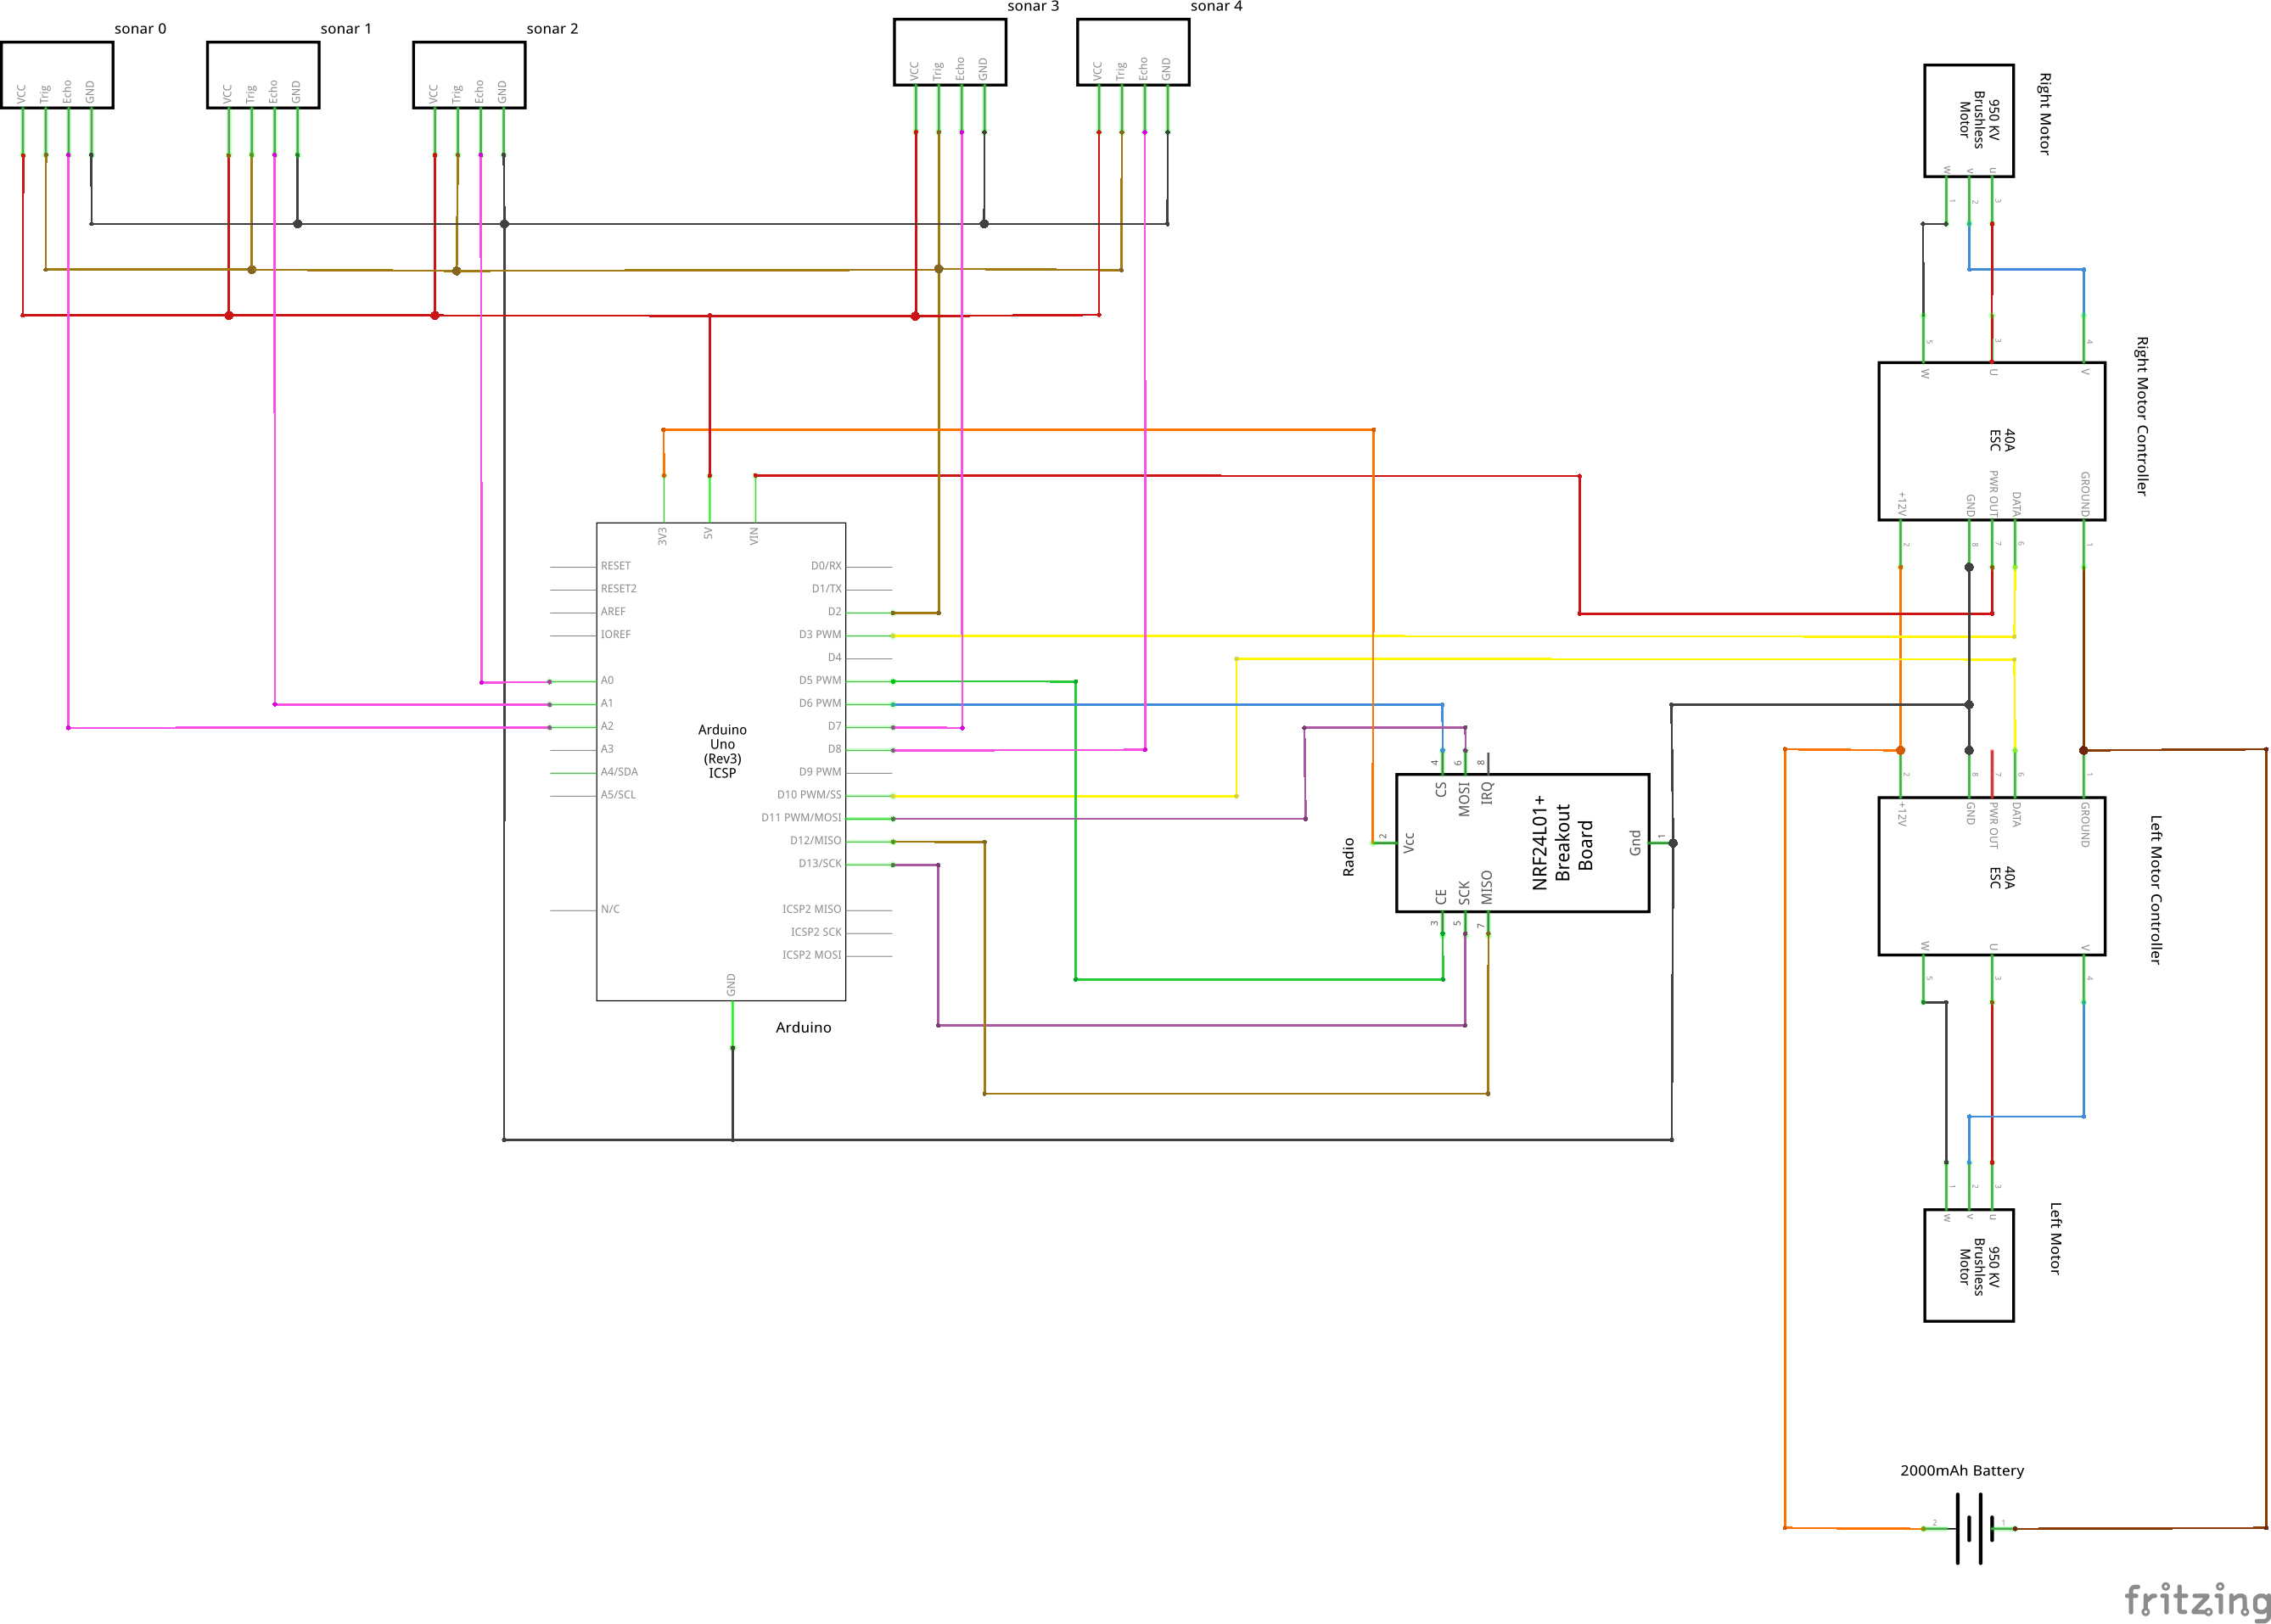
\includegraphics[width= 0.85 \linewidth]{../../Imagens/robot_schem.png}
    \caption{Diagrama Elétrico} %% TODO: é um bom nome??
    \label{fritzing}
  \end{figure}

\section{Subsistema de Comunicação}
Este segmento teve como alicerce a biblioteca denominada RF24, diponível em \cite{nrf_lib}, responsável por todo o controle em baixo nível do 
\textit{transceiver} nRF24L01+.
Foi implementada em C++ e consiste numa única classe, RF24 (vide Fig.\ref{RF24_ClassDiag}), que provê acesso às funcionalidades básicas do 
\textit{transceiver} como controle da potência de transmissão do sinal e escolha do canal a ser utilizado, tanto quanto funções que permitem enviar 
dados por um canal previamente aberto e ler dos canais em que o dispositivo se comporta como receptor; a documentação completa da classe pode ser 
encontrada em \citeonline{RF24_class_doc}.
Assim como todos os códigos de terceiros e programas utilizados nesse projeto, sua utilização é aberta ao público gratuitamente, conforme os termos 
de uso.

Na definição do escopo do projeto, o papel do módulo de radiofrequência seria de simplesmente garantir a segurança e integridade do robô.
Neste caso, uma comunicação \textit{simplex} seria suficiente para cumprir a tarefa.
O módulo transmissor, localizado no acionador remoto, enviava ao robô o nível lógico lido do botão de segurança.
O \textit{transceiver} do robô assumia o papel de receptor e enviava os dados recebidos por comunicação serial ao Arduino, que ordenava a parada dos 
motores caso a mensagem indicasse que o botão estava desligado ou se nenhum pacote fosse detectado num período pré-determinado de 1 segundo.

No entanto, após concluir o sistema de acionamento sem fio, concebeu-se a ideia de sofisticar a utilização do módulo de radiofrequência, 
implementando uma interface de comando capaz de alterar e supervisionar os parâmetros e dados sensoriais do robô, com o intuito de facilitar a etapa 
de testes com o veículo em movimento, objetivando evitar ao máximo a necessidade de reprogramá-lo.

Ao adicionar essa funcionalidade, surge a necessidade de que ambas partes, i.e. robô e sistema de controle remoto, possam receber e enviar 
informações um ao outro.
Como o \textit{transceiver} utilizado tem a funcionalidade de estabelecer comunicação \textit{half-duplex} para cada canal, i.e. bidirecional mas não 
simultaneamente, pois o receptor pode inserir dados no pacote de confirmação de recepção, \textit{acknowledgment packet} \cite{nRF}, e a biblioteca 
RF24 apresenta funções prontas que facilitam o emprego deste recurso, foi possível adicionar essa funcionalidade ao projeto sem a necessidade de 
utilizar dois canais de comunicação.

A interface de comando implementada abrange as seguintes funções:
\begin{itemize}
 \item Ajustar a frequência do PWM de cada um dos motores.
 \item Ajustar a velocidade angular dos motores, que corresponde ao \textit{duty cicle} do sinal de controle, modulado em largura de pulso.
 \item Enviar parâmetros do robô ao controlador remoto: frequência dos PWMs, velocidades dos motores, leituras dos sensores ultrassônicos, 
\textit{status} do botão de segurança de acordo com o veículo.
 \item Energizar os motores na velocidade estipulada enquanto o botão de segurança estiver acionado e não houver obstáculos que representem perigo ao 
robô.
 \item Acionar o sistema de navegação autônoma, também subordinado ao botão de segurança, com tentativas de envio das informações sensoriais e 
comportamentais a cada tomada de decisão do veículo ao controlador remoto sem suspender a movimentação do robô.
 \item Acionar o sistema de navegação autônoma por um número pré-estabelecido de leituras dos sonares, seguido de envio de todos dados coletados ao 
controlador remoto com o robô parado.
\end{itemize}


  \begin{figure}[H]
    \centering
    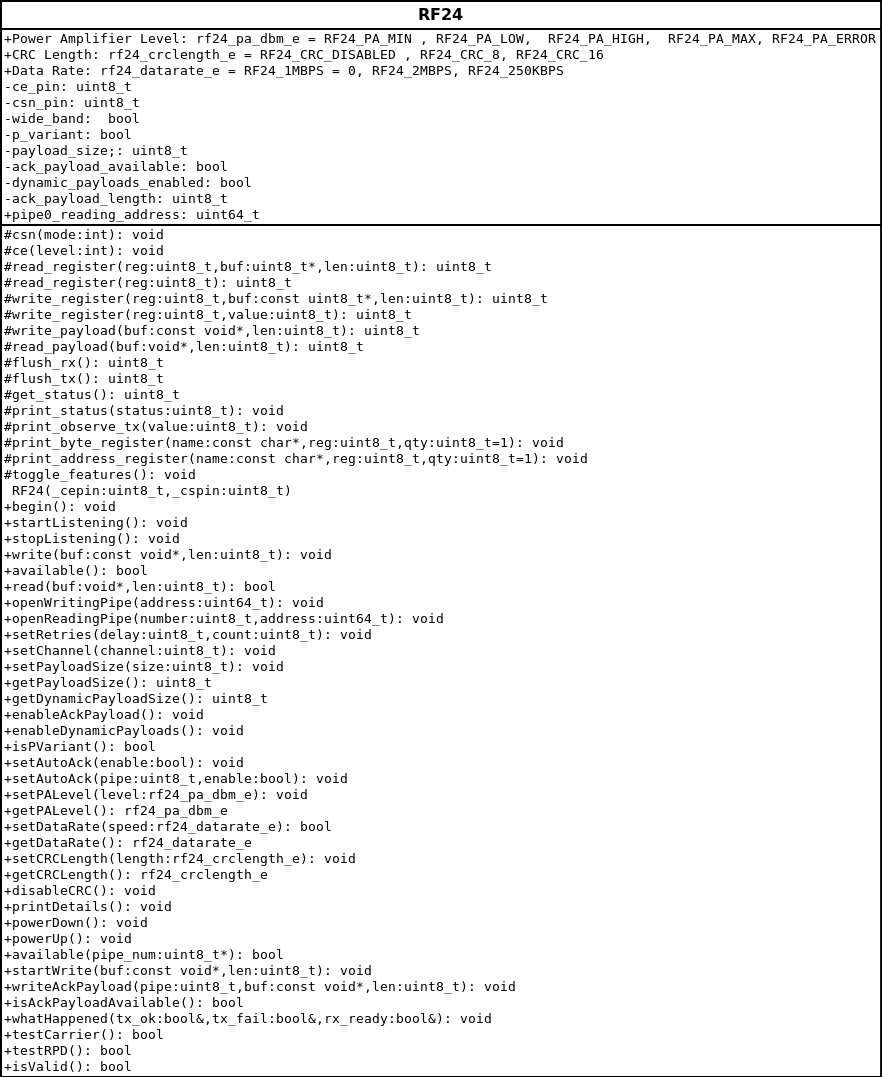
\includegraphics[width=0.5 \linewidth]{../../Imagens/RF24_class.png}
    \caption{Diagrama da Classe RF24} %% TODO certificar se realmente é uma WBS!!!
    \label{RF24_ClassDiag}
  \end{figure}
\section{Subsistema de Navegação} % TODO subsistema ou estratégia de desvio de obstáculos?
Consiste na inteligência  do robô, isto é, trata-se do conjunto de comportamentos adotados pelo veículo, através dos quais ele é capaz de 
desempenhar sua função de desvio de obstáculos. % TODO é realmente necessário falar isso?
Tal qual foi feito em \citeonline{Artigo_3}, a área coberta por um dado sensor ultrassônico foi dividida em três regiões: distante, próxima e perigo.
Quando a leitura de todos os sonares indica região distante, i.e. obstáculos distam mais do que 3 metros, considera-se que o robô 
está seguro e pode andar em velocidade máxima; em futuros trabalhos, corresponderá à situação em que o controle do veículo é cedido ao MOSA.
Caso a medida de algum dos sensores seja menor do que 1 metro - região de perigo - entende-se que o robô está na iminência de uma colisão e deve 
freiar imediatamente.
Quando nenhuma destas situações citadas ocorre, isto é, nenhum dos sonares da matriz está na região de perigo, mas há ao menos um deles que não está 
na região distante, por conseguinte na região próxima, entende-se que há um obstáculo passível de ser contornado.

A estratégia de desvio de obstáculos é semelhante à desenvolvida em \cite{Artigo_1} e define comportamentos bem simples e diretos, como atos reflexos 
nos animais, garantindo rapidez de resposta uma vez que as leituras dos sensores já foram feitas, vide Fig. \ref{ObstAvoid}.
Analisa-se cada um dos cinco sonares quanto à região em que se encontra a barreira identificada: 0 para região distante e 1, próxima;
cada uma das 32 combinações possíveis apresenta um comportamento correspondente: seguir em frente, fazer uma curva aberta, moderada ou brusca.
Na Tabela \ref{IA} utiliza-se \textquoteleft E\textquoteright{} e  \textquoteleft D\textquoteright{} para designar curvas à esquerda e direita, 
respectivamente; enquanto os índices \textquoteleft L\textquoteright{},  \textquoteleft M\textquoteright{} e \textquoteleft F\textquoteright{} 
caracterizam o quão acentuada vai ser a curva: leve, moderada ou forte. % tirar isso daqui e colocar legenda na tabela. 

  \begin{figure}[H]
    \centering
    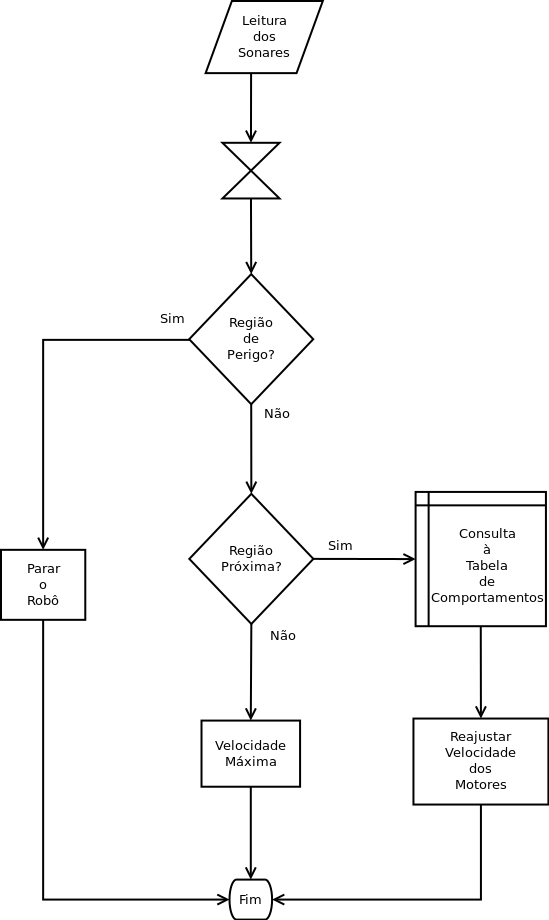
\includegraphics[width=0.5 \linewidth]{../../Imagens/ObstAvoid.png}
    \caption{Fluxograma da Rotina de Desvio de Obstáculos}
    \label{ObstAvoid}
  \end{figure}
  
\section{Integração dos Subsistemas}
Assim que todos os subsistemas foram implementados, testados e operavam isoladamente de maneira satisfatória, foram feitos testes no conjunto, que 
indicaram novos problemas a serem tratados. 
A maioria deles de ordem prática e facilmente contornáveis, no entanto um é digno de nota, pois implicou em uma mudança na disposição física dos 
componentes do veículo que acabou não solucionando o problema. Maiores detalhes, vide seção de Resultados.